\chapter{Les factures}
Les factures sont comme les devis une des fonctionnalités les plus importantes de l'application. De propriétés semblable, il est aussi possible de créer plusieurs factures pour un projet.
\section{Liste des factures\index{Facture!Liste}}
Pour afficher les factures d'un projet il faut, à partir du panneau contenant la liste des projets d'un client, faire un double clic sur le projet en question. La liste affichée contient les factures et les devis du projet sélectionné auparavant.

\section{Ajouter une facture\index{Facture!Ajouter}}
Pour ajouter une facture, il est nécessaire de sélectionner un client dans le panneau central (si l'on est dans la liste des projets ou des factures, la nouvelle facture sera automatiquement ajouté à ce client). Une fois le client selectionné on crée une nouvelle facture en cliquant sur le bouton << Nouvelle facture >> de la barre d'outils ou via le menu << Client $\rightarrow$ Nouvelle facture >>. 
\begin{figure}[H]
	\centering
	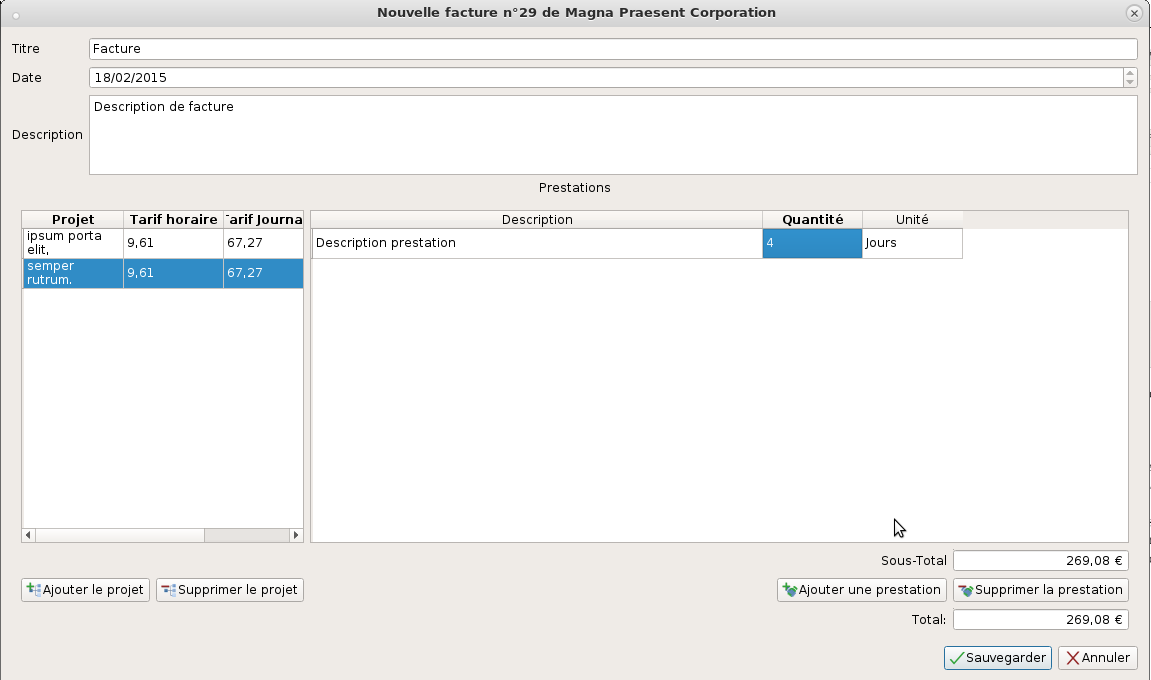
\includegraphics[width=15cm]{screens/creerFacture.png}
	\caption{Créer une nouvelle facture à un projet client}
\end{figure}
Une facture possède un titre à afficher, une date (celle du jour de création du projet), une description et deux tableaux exactement comme lors de la création ou l'édition d'un devis. Le fonctionnement est le même que pour un devis.
\section{Les Prestations\index{Facture!Prestation}}
Les prestations ont exactement le même comportemement que lorsqu'on fait une création ou une édition d'un devis.